\documentclass[
  aps,
  reprint,
  superscriptaddress,
  floatfix,
  nofootinbib,
  longbibliography
]{revtex4-2}

\usepackage{amsmath,amssymb}
\usepackage{graphicx}
\usepackage{xcolor}
\usepackage{tikz}
\usetikzlibrary{calc,positioning,arrows.meta}
\usepackage{hyperref}

\hypersetup{
  colorlinks=true,
  linkcolor=blue,
  citecolor=blue,
  urlcolor=blue
}

% --- convenience macros -------------------------------------------------
\newcommand{\R}{\mathbb{R}}
\newcommand{\E}{\mathbb{E}}
\newcommand{\Prob}{\mathbb{P}}
\newcommand{\Sph}[1]{S^{#1}}
\newcommand{\deff}{d_{\mathrm{eff}}}
\newcommand{\meff}{m_{\mathrm{eff}}}
\newcommand{\sint}{\sigma_{\mathrm{int}}}
\newcommand{\Eint}{E_{\mathrm{int}}}
\newcommand{\T}{^{\mathsf{T}}}
\newcommand{\opnorm}[1]{\lVert #1 \rVert_{\mathrm{op}}}
\newcommand{\norm}[1]{\lVert #1 \rVert}
\newcommand{\ReLU}{\mathrm{ReLU}}

\DeclareMathOperator*{\argmax}{arg\,max}
\DeclareMathOperator{\spanop}{span}
\DeclareMathOperator{\Var}{Var}

\begin{document}

\title{Geometric Limits on Semantic Expressibility: Quantum-Inspired Contexts and Polysemy in Large Language Models}

\author{Karl Svozil}
\email{karl.svozil@tuwien.ac.at}
\affiliation{Institute for Theoretical Physics, TU Wien,
Wiedner Hauptstra\ss{}e 8--10/136, 1040 Vienna, Austria}

\date{\today}

\begin{abstract}
High-dimensional embedding spaces can host many semantic directions
with small mutual overlap. But small overlaps are not zero: when many
directions are jointly active, their residual interference accumulates
and limits what a finite readout channel can recover. We formulate this
as a distinction between \emph{kinetic capacity}---what the geometry
can host---and \emph{epistemic accessibility}---what readout can
recover. The two sides are summarized by
$N\lesssim\exp(c\,\deff\,\varepsilon^{2})$ for coexistence and
$\sint\sim\sqrt{k/\deff}$ for simultaneous readout. Thus dimension acts
not merely as storage capacity but as semantic concurrency bandwidth.
On this geometric foundation we propose a separate hypothesis: some
polysemous tokens may be organized around stable token-associated
reference directions, with sense information carried by low-dimensional
subspaces in their orthogonal complement. The capacity/accessibility
distinction is the main claim; the reference-subspace hypothesis is a stronger,
separately falsifiable empirical proposal.
\end{abstract}

\maketitle

\noindent\textit{Author note.---}
This chapter is adapted and expanded from the preprint
\href{https://doi.org/10.48550/arXiv.2504.13824}{\textit{Semantic
Concurrency Limits in Large Language Models}}.  The present version adds
framing for the Ernst Str\"ungmann Forum volume, cross-chapter connections,
and revisions reflecting the discussions of the Forum.

% ======================================================================
\section{Introduction}
\label{sec:intro}
% ======================================================================

This chapter examines contextual representation in large language models
(LLMs) as part of the volume's broader inquiry into ``quantum thinking.''
Only a minimal orientation to LLM operation is needed here.  Input text is
first divided into tokens, and each token is mapped to an initial vector.
Transformer blocks then use self-attention and feed-forward transformations
to turn those initially context-free vectors into sequence-dependent hidden
states.  An output layer converts the final state into token scores, and a
softmax distribution supports probabilistic next-token selection.  This
compact chain---tokens, embeddings, contextual transformation, and finite
readout---supplies the computational background for the argument below; the
details of pre-training, fine-tuning, reinforcement learning, and
backpropagation are not required.

Current Transformer-based LLMs are classical computational systems.  They
run on classical hardware and use real-valued matrix operations,
normalization, nonlinearities, copying, and generally irreversible updates.
Their reliance on vectors, inner products, high dimension, or probabilistic
output does not by itself make them quantum or even quantum-like.  The more
limited question pursued here is where ordinary high-dimensional geometry
already explains the coexistence and contextual selection of semantic
features, and where a stronger comparison with quantum-like formalisms might
begin.  Such a comparison would have to do more than rename familiar neural
operations: it would need to identify a role for contextual bases or subspaces,
incompatible or noncommuting alternatives, interference, or
measurement-like readout that yields explanatory or predictive value beyond
a classical dynamic-embedding account.

Semantic concurrency makes this boundary concrete.  A model must preserve
many latent possibilities while making only a small, context-selected subset
operationally accessible.  Polysemy is the simplest illustration: the same
token can participate in the meanings of ``river bank'' and ``financial
bank,'' yet the surrounding sequence drives it toward different contextual
representations.  This relation among possibility, context, and readout
connects directly to the volume's recurring themes without implying that the
underlying machine is physically quantum.  It also motivates a separation
between what a representation can geometrically accommodate and what a
finite channel can reliably recover.

Within Part III, the chapter therefore occupies a deliberately intermediate
position.  Chapter~3 supplies the shared vocabulary of state spaces,
contexts, Hilbert-space geometry, and quantum-like representation.
Chapter~7 develops a contrasting route in which classical oscillatory and
wave dynamics can support interference-like computation.  The present
chapter instead asks how far high-dimensional representation, contextual
selection, and readout can take a classical artificial language system.
Chapter~9 places these results beside neural systems, embodiment, meaning,
and the limits of the quantum analogy.  Chapter~13 and Bridge~C provide the
corresponding standards for model comparison and evidence: an analogy should
be sharpened into explicit structure and then into a discriminative test
before it is treated as an explanation.

The claims below consequently occupy different rungs of that evidential
ladder.  Concentration of measure and exponential packing are standard
results of high-dimensional geometry.  Their use to describe semantic
capacity, together with the accumulated-interference estimate, is a formal
model of classical representation subject to stated assumptions about
effective dimension and coactivation.  The reference-subspace organization is
a stronger empirical hypothesis about LLM internals and is tested against
classical controls.  The comparison with quantum contextuality remains a
limited structural correspondence; no physical quantumness, Born-rule
dynamics, or semantic Kochen--Specker theorem is inferred.

A finite-dimensional activation space faces a simple tension. High
dimension lets many semantic features coexist as nearly orthogonal
directions. Finite readout prevents too many of them from being
simultaneously recovered from one channel. This chapter makes that
tension quantitative.

The two sides obey different scalings. On the capacity side,
concentration of measure permits exponentially many candidate semantic
directions with pairwise overlap at most $\varepsilon$,
%
\begin{equation}
\label{eq:intro-capacity}
N\lesssim \exp(c\,\deff\,\varepsilon^{2}).
\end{equation}
%
On the readout side, the same small residual overlaps add in quadrature
over an active set of size $k$, giving an interference scale
%
\begin{equation}
\label{eq:intro-readout}
\sint\sim\sqrt{k/\deff}.
\end{equation}
%
The first relation is an existential packing estimate. The second is a
typical-case readout-noise estimate. Together they say that dimension
is a \emph{semantic concurrency bandwidth}: it does not mainly limit how
many meanings can be geometrically stored, but how many independently
recoverable semantic components can be jointly active.

Polysemy is the cleanest example. A single lexical item, such as
``bank'', can access several mutually exclusive meanings, only one of
which is selected in a given context. The same tension appears more
generally in feature superposition, role binding, and compositional
semantics~\cite{mikolov2013}: many latent semantic degrees of freedom
must coexist, while only a context-selected subset is read out. We use
polysemy as a controlled entry point because it makes contextual
selection explicit. In lexical semantics, polysemy is distinguished
from homonymy by the relatedness of senses~\cite{pustejovsky1995}.
Modern Transformer-based LLMs implement contextual selection through
dynamic contextual embeddings: a token representation is repeatedly
transformed by self-attention and MLP layers as it absorbs information
from its sentential environment~\cite{Vaswani-2017-Attention}.

The chapter makes two claims. The first is the geometric capacity claim:
concentration permits large semantic capacity, while accumulated
interference limits simultaneous accessibility. This claim is
architecture-independent. The second is a stronger organizational
hypothesis: for some canonically polysemous tokens, readout may be
structured relative to a stable token-associated \emph{reference direction},
with sense information carried by low-dimensional subspaces in its
orthogonal complement. The reference-subspace hypothesis is not implied by
concentration geometry. It is an empirical proposal, and
Sec.~\ref{sec:predictions} states how it can fail.

A serious caveat is effective dimension. Trained representations are
often anisotropic: they occupy a narrow cone rather than the full
ambient space. The dimension controlling concentration is therefore
not necessarily the raw embedding dimension $d$, but an effective
dimension $\deff$. If $\deff$ is small, the capacity claim weakens
accordingly. For example, at $\deff\sim 50$ and $\varepsilon=0.1$, the
exponent $c\deff\varepsilon^{2}$ is only a small constant. The framework
therefore applies to the approximately isotropic geometry actually used
by the representation, possibly after whitening or restriction to a
participation subspace. Determining which layers, models, and
preprocessing regimes admit a meaningful $\deff$ is an empirical
priority.

The reference-subspace hypothesis has a narrower domain. It is meant for
canonically polysemous tokens with established sense inventories, such
as WordNet-, OntoNotes-, SemCor-, or WiC-style sense
distinctions~\cite{pilehvar2019wic} with enough contextual instances
for testing. Failure on a representative sample, against the controls
in Sec.~\ref{sec:predictions}, would count against a privileged token
reference direction even
if the broader capacity/accessibility picture survives.

The proposal is adjacent to the superposition hypothesis in mechanistic
interpretability~\cite{elhage2022superposition}, according to which neural networks
represent more features than they have neurons by packing features into
nearly orthogonal directions. The present chapter separates the
geometric background from a possible semantic organization within it.
The general superposition picture concerns an overcomplete dictionary
of feature directions and sparse active sets. The reference-subspace picture adds
the more specific possibility that some contextual readout is organized
around stable token-associated directions.

Section~\ref{sec:concentration} develops the capacity framework:
quasi-orthogonality, L\'evy's lemma, exponential packing, and the
kinetic/epistemic distinction. Section~\ref{sec:reference} introduces the
reference-subspace hypothesis and its relation to dynamic contextual
embeddings. Section~\ref{sec:attention} connects the picture to
attention as soft routing rather than literal basis reconstruction.
Section~\ref{sec:discussion} discusses superposition, sparse
autoencoders, limitations, empirical tests, and the limited quantum
analogy.

{Notation.}
Throughout, $\R^{d}$ is Euclidean $d$-space with inner product $u\T v$
and norm $\norm{v}=\sqrt{v\T v}$; $\Sph{d-1}=\{v\in\R^{d}:\norm{v}=1\}$
is the unit sphere; $I$ is the identity matrix; $\opnorm{\cdot}$ is the
operator norm; $A\succeq0$ means positive semidefinite; and $\Prob$ and
$\E$ denote probability and expectation under the uniform measure on
the relevant sphere unless stated otherwise. Universal positive
constants are denoted $c,c'$, possibly changing from line to line.
The symbol $\deff$ denotes the effective dimension controlling
concentration in the representation being probed.

% ======================================================================
\section{Concentration geometry and capacity}
\label{sec:concentration}
% ======================================================================

This section is architecture-independent. It gives the geometric
capacity constraint on which the later reference-subspace hypothesis builds.

\subsection{Quasi-orthogonality}
\label{sec:quasiortho}

Let $w_{1},\dots,w_{N}\in\R^{d}$ be unit feature directions. Strict orthogonality,
$w_i\T w_j=0$ for $i\neq j$, allows at most $N=d$ such vectors. Semantic
encoding does not require exact orthogonality. It requires approximate
distinguishability. We therefore call a family
$\varepsilon$-quasi-orthogonal if
%
\begin{equation}
\label{eq:quasiortho}
|w_i\T w_j|\le \varepsilon,\qquad i\neq j .
\end{equation}
%
This is the relevant notion for high-dimensional feature storage:
small overlap is tolerable, provided readout can absorb the resulting
interference.

\subsection{L\'evy's lemma and linear overlaps}
\label{sec:levy}

High-dimensional spheres make quasi-orthogonality generic.

%\paragraph*{Heuristic concentration argument.}
The mechanism is already visible before invoking the formal lemma.  Let
\[
        x=(x_1,\ldots,x_d)\in\R^d
\]
be a unit vector chosen without a preferred direction.  Then
\[
        x_1^2+\cdots+x_d^2=1 .
\]
Rotational invariance suggests that the norm is spread over the available
coordinates, so a typical coordinate weight is of order $1/d$.  Now fix a
unit direction $u$.  By rotational invariance one may choose coordinates so
that $u=e_1$.  The squared overlap with the random direction is then
\[
        |u\T x|^2=x_1^2 .
\]
Thus the overlap with any fixed direction is typically of order $d^{-1/2}$
in amplitude, or $1/d$ in squared amplitude.  A macroscopic overlap
$|u\T x|>\varepsilon$ therefore requires one coordinate to carry an
anomalously large fraction of the total norm.  In high dimension such an
event is exponentially unlikely.

The same intuition appears particularly transparently in the complex
Hilbert-space analogue.  If $\psi\in\mathbb{C}^D$ is Haar-random and
$\phi$ is fixed, unitary invariance permits the choice $\phi=e_1$, so
\[
        |\langle\phi,\psi\rangle|^2=|\psi_1|^2 .
\]
For a Haar-random complex unit vector the exact tail is
\[
        \Prob\{ |\langle\phi,\psi\rangle|^2\geq\eta\}
        =(1-\eta)^{D-1}
        \leq \exp[-(D-1)\eta] .
\]
For real embedding vectors the analogous spherical concentration estimate
has the operative scaling
\[
        \Prob\{ |u\T x|>\varepsilon\}
        \lesssim \exp(-c d\varepsilon^2)
\]
for a universal constant $c>0$.  Consequently, if $N$ random directions are
sampled, a union-bound estimate gives a probability at most of order
$N^2\exp(-c d\varepsilon^2)$ that some pair has overlap larger than
$\varepsilon$.  Hence $N$ may grow exponentially in $d\varepsilon^2$ while
all pairwise overlaps remain small with high probability.  This is the
heuristic core of the exponential quasi-orthogonal capacity derived below.

L\'evy's lemma makes this intuition precise.  If $f:\Sph{d-1}\to\R$
is $L$-Lipschitz, then
%
\begin{equation}
\label{eq:levy}
\Prob\bigl(|f(v)-\E f|\ge\delta\bigr)
 \le
2\exp\!\left(-\frac{c\,d\,\delta^{2}}{L^{2}}\right),
\end{equation}
%
for a universal $c>0$~\cite{ledoux2001concentration,milman1986asymptotic}. Apply this to the
linear functional $f_u(v)=u\T v$. It is $1$-Lipschitz and has mean zero
by symmetry. Hence
%
\begin{equation}
\label{eq:overlap}
\Prob\bigl(|u\T v|\ge\varepsilon\bigr)
 \le 2\exp(-c\,d\,\varepsilon^{2}).
\end{equation}
%
For normalized surface measure one obtains the explicit form
$2\exp(-(d-1)\varepsilon^{2}/2)$~\cite{ledoux2001concentration}. Thus two random
unit vectors are nearly orthogonal with high probability, and typical
overlap amplitudes scale as $d^{-1/2}$.

In trained models, $d$ should be replaced by $\deff$, the dimension
actually controlling concentration. Anisotropy, low intrinsic
dimension, or a narrow activation cone reduce $\deff$. Whitening or
projection to a participation subspace may increase the effective
dimension relevant for the analysis.

{Relation to Johnson--Lindenstrauss.}
The Johnson--Lindenstrauss lemma preserves pairwise distances among
$n$ points after projection to dimension
$k=O(\varepsilon^{-2}\log n)$~\cite{johnson-1984}. It is driven by the
same concentration phenomenon as Eq.~\eqref{eq:overlap}; indeed JL can
be derived from sphere concentration applied to projection
norms~\cite{Dasgupta-2003}. Here L\'evy's lemma is the more direct tool:
the issue is not projecting a finite dataset, but the typical overlap
between semantic directions in the representation space.

\subsection{Exponential packing}
\label{sec:packing}

Sample $N$ unit vectors independently and uniformly from
$\Sph{d-1}$. By Eq.~\eqref{eq:overlap} and a union bound over pairs,
%
\begin{equation}
\label{eq:unionbound}
\Prob\bigl(\exists\,i\neq j:\ |w_i\T w_j|\ge\varepsilon\bigr)
 < N^{2}\exp(-c\,\deff\,\varepsilon^{2}).
\end{equation}
%
This probability is below one, and hence an
$\varepsilon$-quasi-orthogonal family exists, provided
%
\begin{equation}
\label{eq:packing}
N < \exp\!\left(\frac{c}{2}\,\deff\,\varepsilon^{2}\right).
\end{equation}
%
This is the kinetic capacity estimate: in high effective dimension,
many candidate semantic directions can coexist with small pairwise
overlap.

The estimate controls pairwise overlap only. It does not guarantee that
a large collection of feature directions is well-conditioned. By Gershgorin,
$|w_i\T w_j|\le\varepsilon$ gives only
$\opnorm{G-I}\le(n-1)\varepsilon$ for an $n$-element Gram matrix, which
is useless when $n$ is large. Joint readout therefore needs a
separate conditioning assumption, introduced in Sec.~\ref{sec:gated}.

\subsection{Kinetic capacity versus epistemic accessibility}
\label{sec:kinetic-epistemic}

The packing bound says what can coexist. It does not say what can be
read. We call the coexistence supply \emph{kinetic semantic capacity}.
We call the recoverable subset \emph{epistemic semantic accessibility}.
The distinction is the central point of the chapter.

Let $N$ candidate features be represented by unit directions
$w_1,\dots,w_N\in\R^{\deff}$. In a given context, suppose an active set
$S$ of size $k$ contributes amplitudes $x_j$, producing
%
\begin{equation}
\label{eq:hidden}
h=\sum_{j\in S}x_j w_j .
\end{equation}
%
A linear readout of feature $i$ gives
%
\begin{equation}
\label{eq:readout}
w_i\T h
=
x_i+
\sum_{\substack{j\in S\\ j\neq i}}
x_j\,w_i\T w_j .
\end{equation}
%
The first term is signal; the second is interference. For random
incoherent directions,
%
\begin{equation}
\label{eq:moments}
\E[w_i\T w_j]=0,
\qquad
\Var(w_i\T w_j)\simeq \frac{1}{\deff}.
\end{equation}
%
Thus, conditional on the active amplitudes,
%
\begin{equation}
\label{eq:intvar}
\Var\!\left(
\sum_{\substack{j\in S\\ j\neq i}}
x_j\,w_i\T w_j
\right)
\simeq
\frac{1}{\deff}
\sum_{\substack{j\in S\\ j\neq i}}x_j^2 .
\end{equation}
%
For amplitudes of order unity,
%
\begin{equation}
\label{eq:sint}
\sint\sim\sqrt{\frac{k}{\deff}} .
\end{equation}
%
This is the readout bottleneck. Concentration lets many directions
coexist because their overlaps are small. But readout sees the
\emph{sum} of many small overlaps. Reliable recovery requires
%
\begin{equation}
\label{eq:snr}
\sqrt{\frac{k}{\deff}}\ll \Delta,
\end{equation}
%
where $\Delta$ is the relevant decision margin. Equivalently,
%
\begin{equation}
\label{eq:dual}
\text{kinetic: }N\lesssim\exp(c\,\deff\,\varepsilon^{2}),
\qquad
\text{epistemic: }k\lesssim\deff\,\Delta^{2}.
\end{equation}
%
The first is storage-like coexistence. The second is simultaneous
accessibility. A model may host many more features than it can jointly
read.

Figure~\ref{fig:toy-scalings} gives a minimal synthetic illustration of
this distinction. The simulation is not intended as a model of a trained
language model. It is only a null model for the concentration geometry:
random unit directions in an effective dimension $\deff$ can coexist in
large quasi-orthogonal families, while simultaneous linear readout
accumulates the residual overlaps of the active directions. Deviations
from this null model in trained representations would themselves be
informative, reflecting anisotropy, learned feature alignment, nonlinear
readout, or coactivation-dependent orthogonalization.

\begin{figure*}[t]
\centering
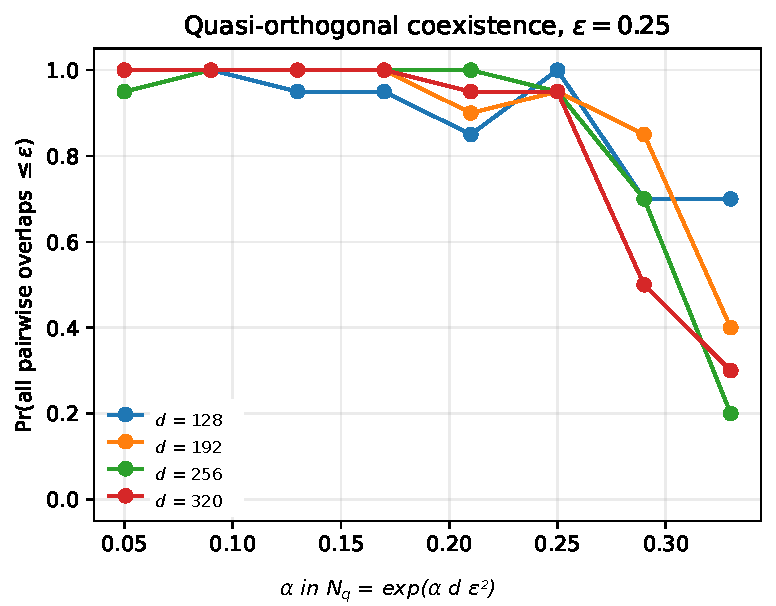
\includegraphics[width=0.48\textwidth]{2026-llm-quasi_orthogonal_coexistence.pdf}
\hfill
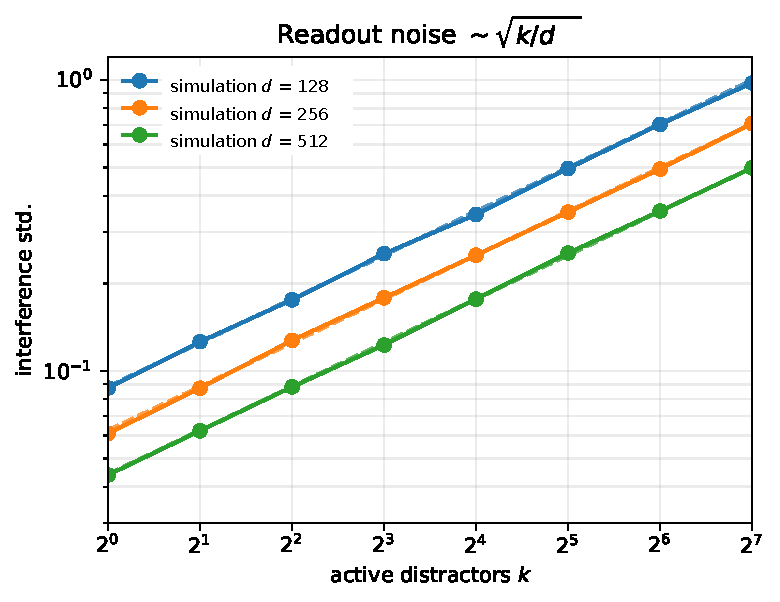
\includegraphics[width=0.48\textwidth]{2026-llm-readout_interference.pdf}
\caption{%
Synthetic geometry checks for the capacity/accessibility distinction.
Left: random unit directions in dimension $\deff$ are sampled with
$N=\exp(\alpha\,\deff\,\varepsilon^{2})$ and tested for
$\varepsilon$-quasi-orthogonality. For sufficiently small $\alpha$,
large families coexist with high probability, illustrating the
exponential packing side of Eq.~\eqref{eq:dual}. Right: for a fixed
target direction, $k$ random distractor directions are simultaneously
active with random signs. The standard deviation of the readout
interference follows the predicted scale
$\sint\sim\sqrt{k/\deff}$, illustrating the accessibility side of
Eq.~\eqref{eq:dual}. Both panels use random isotropic vectors and should
be read as a geometric null model rather than as measurements on a
trained language model.
}
\label{fig:toy-scalings}
\end{figure*}

This also clarifies the relation to compressed sensing. Stable recovery
of a $k$-sparse vector in an $N$-dimensional feature dictionary from
$m$ measurements typically requires
$m\gtrsim Ck\log(N/k)$ under suitable incoherence or restricted-isometry
assumptions~\cite{donoho2006compressed,candes2006robust,foucart2013mathematical}. In an idealized
isotropic residual stream, one may identify $m$ with $\deff$; in trained
models the effective representation dimension and effective readout
dimension may differ. The compressed-sensing analogy is therefore
diagnostic, not literal.

% ======================================================================
\section{Token reference directions and sense subspaces}
\label{sec:reference}
% ======================================================================

The previous section established an architecture-independent capacity
constraint. We now ask a more speculative question: does a trained model
organize the contextual states of some polysemous tokens relative to a
stable token-associated reference subspace? This hypothesis is not implied
by concentration geometry, and it is separately falsifiable.

The notation distinguishes mathematical types and roles. For a token $t$
and a sense context $C$:
%
\begin{itemize}
\item $r_t\in\R^d$ is a unit candidate token reference vector;
\item $\mathcal R_t\subset\R^d$ is the token reference subspace;
\item $S_{t,C}\subset\mathcal R_t^\perp$ is a low-dimensional sense
subspace;
\item $u_{t,C,j}\in S_{t,C}$ are vectors spanning that sense subspace;
\item $h_\ell(t\mid x)\in\R^d$ is an observed contextual hidden state.
\end{itemize}
%
Thus $r_t$, $u_{t,C,j}$, and $h_\ell(t\mid x)$ are vectors, whereas
$\mathcal R_t$ and $S_{t,C}$ are subspaces. The $w_i$ used in
Sec.~\ref{sec:concentration} have a separate role: they are generic feature
directions in the capacity calculation and are not reused as sense labels.

\subsection{The reference-subspace hypothesis}
\label{sec:reference-hypothesis}

In the simplest version, let $r_t$ be a candidate unit direction and set
%
\begin{equation}
\label{eq:reference-direction}
\mathcal R_t=\spanop\{r_t\}.
\end{equation}
%
Empirically, $r_t$ could be the normalized static input embedding, a
normalized mean contextual embedding, or a learned token-specific probe
direction. It is simply a hypothesized context-stable reference for token
identity. It is not a mechanical or dynamical object.
Any state can be decomposed relative to any direction, so the decomposition
alone has no empirical content. The claim is that a token-associated
$\mathcal R_t$ exposes sense structure better than matched control
directions or subspaces.

For each context or sense label $C$, define a low-dimensional subspace
%
\begin{equation}
\label{eq:sense-subspace}
S_{t,C}=\spanop\{u_{t,C,1},\dots,u_{t,C,q_C}\}
\subset\mathcal R_t^\perp,
\qquad q_C\ll\deff .
\end{equation}
%
For example, finance, river-edge, and aircraft-tilt uses of ``bank'' may
correspond to different subspaces $S_{\mathrm{bank},C}$ inside the common
orthogonal carrier $\mathcal R_{\mathrm{bank}}^\perp$. A word sense is not
a single vector: topic, syntax, selectional preferences, and world knowledge
may require several spanning directions $u_{t,C,j}$.

The reference object may itself require more than one direction. In that
case define
%
\begin{equation}
\label{eq:reference-subspace}
\mathcal R_t=
\spanop\{r_{t,1},\dots,r_{t,p}\},
\qquad p\ge1,
\end{equation}
%
and require
%
\begin{equation}
\label{eq:multi-sense-subspace}
S_{t,C}\subset\mathcal R_t^\perp .
\end{equation}
%
Equation~\eqref{eq:reference-direction} is the special case $p=1$.
The analogy with interlinked quantum contexts is limited to a pattern of
sharing. In quantum logic, different contexts can share one or more
observables or projections; finite-dimensional examples with two shared
observables are known~\cite{svozil:040102}. In the semantic model,
$\mathcal R_t$ is instead a common token-associated reference subspace, and
the sense-specific subspaces lie in its orthogonal complement. No
noncommutativity or quantum probability is implied by
Eqs.~\eqref{eq:reference-subspace}--\eqref{eq:multi-sense-subspace}.

The low-rank assumption is empirical. It predicts that dominant
within-sense variation is low-dimensional after projection onto
$\mathcal R_t^\perp$. This is compatible with evidence that contextualized
embeddings can separate word senses, but it is stronger: it asks whether
such separation is privileged relative to a token-associated reference
subspace~\cite{wiedemann2019does,scarlini2020ares}.

\subsection{Projection and gated subspace readout}
\label{sec:gated}

Let $h(x)\in\R^d$ be a contextual state and let $P_t$ be the orthogonal
projector onto $\mathcal R_t$. The two components are
%
\begin{align}
\label{eq:reference-decomp}
h(x)&=h_{\rm ref}(x)+h_\perp(x),\\
h_{\rm ref}(x)&=P_t h(x),\nonumber\\
h_\perp(x)&=(I-P_t)h(x)\in\mathcal R_t^\perp.\nonumber
\end{align}
%
For the one-dimensional case, $P_t=r_t r_t\T$ and the scalar
$a_t(x)=r_t\T h(x)$ measures the component along the reference direction.
The hypothesis is that most sense-disambiguating variation is present in
$h_\perp(x)$, not that the projection formula itself is special.

Readout inside $S_{t,C}$ also requires the spanning vectors to be
well-conditioned. Let
%
\begin{equation}
U_{t,C}=[\,u_{t,C,1}\ \cdots\ u_{t,C,q_C}\,],
\qquad
G_{t,C}=U_{t,C}\T U_{t,C}.
\end{equation}
%
The columns of $U_{t,C}$ span $S_{t,C}$; $U_{t,C}$ is a matrix, not an
additional semantic vector. We call it $\rho$-well-conditioned if
%
\begin{equation}
\label{eq:rho-stable}
\opnorm{G_{t,C}-I}\le\rho<1.
\end{equation}
%
Then
%
\begin{equation}
\label{eq:dual-spanning}
\widetilde U_{t,C}=U_{t,C}G_{t,C}^{-1}
\end{equation}
%
is a dual spanning matrix and satisfies
$\opnorm{\widetilde U_{t,C}}\le(1-\rho)^{-1/2}$. Near-degenerate spanning
sets amplify readout noise, so the model requires $\rho$ comfortably below
one. The corresponding coordinates are
%
\begin{equation}
\label{eq:alpha}
\alpha_{t,C}(x)=\widetilde U_{t,C}\T h_\perp(x)
\in\R^{q_C}.
\end{equation}
%

A simple sense score is
%
\begin{equation}
\label{eq:sense-score}
s_{t,C}(x)=g_t(a_t(x))\,f_{t,C}(h_\perp(x)),
\end{equation}
%
where $g_t\ge0$ gates engagement with the token reference direction and
$f_{t,C}\ge0$ measures fit to the sense subspace. One possible choice is
$f_{t,C}=\norm{\alpha_{t,C}(x)}^2$; a learned positive quadratic form is
another. The selected sense label is
%
\begin{equation}
\label{eq:selected-sense}
C^*(x)=\argmax_C s_{t,C}(x).
\end{equation}
%
The empirical content is the proposed separation of roles: the reference
component tracks token identity or engagement, while the orthogonal
component contains sense-disambiguating information. If no token-associated
$\mathcal R_t$ exposes sense structure better than matched random,
frequency-controlled, or layer-matched subspaces, the hypothesis fails.

Figure~\ref{fig:reference-subspace} illustrates these objects without
introducing extra vector symbols.

\begin{figure}[t]
\centering
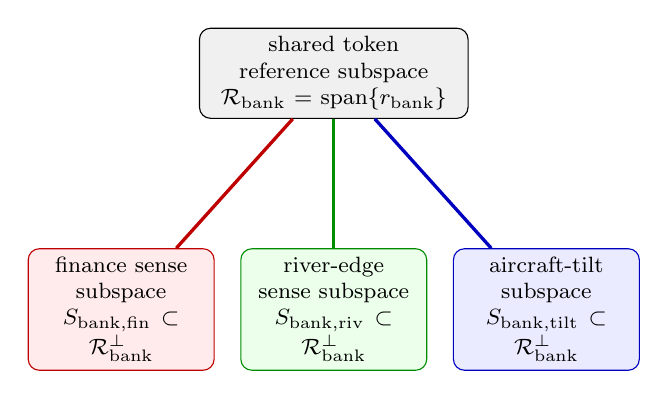
\begin{tikzpicture}[
    box/.style={draw, rounded corners, align=center, font=\footnotesize,
                text width=2.15cm, minimum height=1.05cm, inner sep=3pt},
    ref/.style={box, fill=gray!12, text width=3.2cm},
    conn/.style={very thick}]
\node[ref] (ref) at (0,1.8)
{shared token\\reference subspace\\
$\mathcal R_{\rm bank}=\spanop\{r_{\rm bank}\}$};

\node[box, draw=red!75!black, fill=red!8] (fin) at (-2.7,-1.2)
{finance sense subspace\\
$S_{{\rm bank},{\rm fin}}\subset\mathcal R_{\rm bank}^{\perp}$};

\node[box, draw=green!55!black, fill=green!8] (riv) at (0,-1.2)
{river-edge sense subspace\\
$S_{{\rm bank},{\rm riv}}\subset\mathcal R_{\rm bank}^{\perp}$};

\node[box, draw=blue!75!black, fill=blue!8] (tilt) at (2.7,-1.2)
{aircraft-tilt subspace\\
$S_{{\rm bank},{\rm tilt}}\subset\mathcal R_{\rm bank}^{\perp}$};

\draw[conn, red!75!black] (ref) -- (fin);
\draw[conn, green!55!black] (ref) -- (riv);
\draw[conn, blue!75!black] (ref) -- (tilt);
\end{tikzpicture}
\caption{%
Organization proposed by the reference-subspace hypothesis for the
polysemous token ``bank.'' This is a relationship diagram, not a coordinate
plot. The central box is the one-dimensional reference subspace
$\mathcal R_{\rm bank}=\spanop\{r_{\rm bank}\}$; the three outer boxes are
entire low-dimensional sense subspaces, not individual vectors. All three
lie in the common carrier $\mathcal R_{\rm bank}^{\perp}$. In the
multi-direction version, $\mathcal R_{\rm bank}$ has dimension $p>1$, but
the carrier remains its orthogonal complement. The undirected lines indicate
this common-reference relationship; they do not denote maps or causal flow.
}
\label{fig:reference-subspace}
\end{figure}

\subsection{Packing sense subspaces in a shared orthogonal carrier}
\label{sec:grassmann}

The vector packing bound extends to low-dimensional subspaces. Fix a unit
reference vector $r_0\in\Sph{d-1}$ and let $m=d-1$. For $1\le q\ll m$ and
any fixed threshold $\mu>2\sqrt{q/m}$, there exist $q$-dimensional
subspaces $S_1,\dots,S_M\subset r_0^\perp$ such that
%
\begin{equation}
\label{eq:grassmann-coherence}
\opnorm{U_a\T U_b}\le \mu,\qquad a\neq b,
\end{equation}
%
where $U_a,U_b\in\R^{m\times q}$ are orthonormal basis matrices, and
%
\begin{equation}
\label{eq:grassmann-count}
M\ge \exp(c_{\mu,q}m)
\end{equation}
%
for some positive $c_{\mu,q}$.

This is a standard Grassmannian packing consequence of concentration on
Stiefel and Grassmann manifolds~\cite{szarek1982nets,conway1996packings}.
For two independent Haar-random $q$-planes, the singular values of $U\T V$
are the cosines of their principal angles. In the regime $q\ll m$, the
largest principal correlation is of order
$\sqrt{q/m}$~\cite{chikuse2003statistics,absil2006condition,edelman1998random}.
A union bound over sampled subspaces then gives an exponential packing.

For trained representations this statement must be read inside an
approximately isotropic effective carrier. If
$\dim(\mathcal R_t)=p$, its effective dimension is
$\meff=\deff-p$, not necessarily the raw ambient dimension minus $p$.
Without such an effective carrier, the Haar-random subspace model is not a
good description of activation geometry.

\subsection{Relation to dynamic contextual embeddings}
\label{sec:dynamic}

Transformers already handle polysemy dynamically. The hidden state
$h_\ell(t\mid x)$ of token $t$ at layer $\ell$ depends on context $x$.
The reference-subspace hypothesis is not an alternative architecture; it is
a proposed organization of these observed trajectories.

Given a candidate reference subspace $\mathcal R_t$ and its projector $P_t$,
write
%
\begin{align}
\label{eq:layer-decomp}
h_\ell(t\mid x)
&=P_t h_\ell(t\mid x)+z_\ell(t,x),\\
z_\ell(t,x)&=(I-P_t)h_\ell(t\mid x)
\in\mathcal R_t^\perp.\nonumber
\end{align}
%
The decomposition is automatic; the hypothesis is not. It predicts that
$P_t h_\ell(t\mid x)$ tracks token identity or engagement, while
$z_\ell(t,x)$ carries most sense-disambiguating information. Sense labels
should be more separable in $\mathcal R_t^\perp$ than in the orthogonal
complements of matched control subspaces. For each sense $C$, the projected
states $z_\ell(t,x)$ should also concentrate near the low-dimensional
subspace $S_{t,C}\subset\mathcal R_t^\perp$.

Thus the critical question is not whether contextual embeddings move; they
do. It is whether their sense-relevant movement has a privileged
organization relative to a token-associated reference subspace.

\begin{table*}[ht]
\caption{Dynamic contextual embeddings versus the reference-subspace
hypothesis.}
\label{tab:two-views}
\centering
\begin{minipage}{0.72\textwidth}
\begin{ruledtabular}
\begin{tabular}{@{}ll@{}}
Dynamic description & Reference-subspace hypothesis \\
\colrule
Token state changes by context and layer & State is projected relative to $\mathcal R_t$ \\
Layer activation carries context & $\mathcal R_t^\perp$ contains sense variation \\
Polysemy by vector deformation & Polysemy by context-conditioned subspaces \\
Resource is depth and width & Resource is quasi-dimensionality \\
Limit is activation bottleneck & Limit is interference/accessibility \\
\end{tabular}
\end{ruledtabular}
\end{minipage}
\end{table*}

% ======================================================================
\section{Attention and latent context selection}
\label{sec:attention}
% ======================================================================

A standard attention head computes
%
\begin{equation}
\label{eq:attention}
h'=\sum_j\alpha_j\nu_j,
\qquad
\alpha_j=
\frac{\exp(q\T k_j/\sqrt d)}
{\sum_{j'}\exp(q\T k_{j'}/\sqrt d)} .
\end{equation}
%
Keys and values are produced by different learned maps, so value vectors
are not generally coefficients of a dual basis for the key vectors.
Attention is therefore not literal basis reconstruction.

The useful analogy is softer. Attention routes information: it amplifies
some contextual directions and suppresses others. In the terminology of
Sec.~\ref{sec:reference}, this resembles context-dependent subspace
selection. A literal basis-reconstruction interpretation would require
additional constraints, such as approximately Parseval keys and values
implementing the corresponding dual reconstruction. We do not assume this.

A compact latent-variable version is
%
\begin{equation}
\label{eq:latent}
p(y\mid x,t)=\sum_C p(y\mid x,t,C)\,p(C\mid x,t),
\end{equation}
%
where $t$ is the token being disambiguated, $y$ is a possible output token,
and $C$ indexes candidate sense contexts. One may model
%
\begin{equation}
\label{eq:context-temp}
p(C\mid x,t)=
\frac{\exp(s_{t,C}(x)/T)}
{\sum_{C'}\exp(s_{t,C'}(x)/T)} ,
\end{equation}
%
with $s_{t,C}$ the gated score of Eq.~\eqref{eq:sense-score}. This is not
a claim about the literal implementation of decoding in current LLMs:
standard temperature acts on token logits, not on explicit latent
sense labels. The point is only that ambiguity can be represented as a
distribution over possible sense contexts rather than as a single fixed
interpretation.

% ======================================================================
\section{Discussion}
\label{sec:discussion}
% ======================================================================

The main proposal is the capacity/accessibility distinction. The
reference-subspace hypothesis is one possible organization within that
constraint, not a consequence of it.

\subsection{Relation to superposition and sparse autoencoders}
\label{sec:superposition}

The superposition hypothesis holds that neural networks represent more
features than they have neurons by packing features into nearly
orthogonal directions~\cite{elhage2022superposition,bricken2023monosemanticity}. The concentration
estimate~\eqref{eq:overlap} gives the kinetic side of that picture:
many directions can coexist. Equation~\eqref{eq:sint} gives the
epistemic side: many jointly active features create interference of
scale $\sqrt{k/\deff}$. Sparsity is therefore not an implementation
detail; it is necessary for readout.

Sparse autoencoders (SAEs) give a concrete empirical interface. They
approximate layer activations as sparse expansions over learned decoder
directions, making the $w_i$ of Eq.~\eqref{eq:hidden} measurable
objects rather than hypothetical features. Recent work has scaled SAEs,
studied SAE feature geometry, and automated interpretation of large
numbers of latents~\cite{gao2025scaling,li2025geometry,paulo2025automatically,shu2025survey}. In the
present framework, SAE decoder directions can test the
capacity/accessibility prediction, while sense-conditioned SAE
activation clusters can test the stronger reference-subspace hypothesis.

\subsection{A coactivation-weighted capacity limit}
\label{sec:capacity-limit}

The active-set size $k$ is a crude summary. A more refined description
uses the coactivation graph
%
\begin{equation}
\label{eq:coactivation}
A_{ij}=\Prob(i,j\text{ active}).
\end{equation}
%
If active amplitudes have, conditional on coactivation, zero mean and
pairwise uncorrelated signs, then cross terms cancel in expectation and
feature $j$ contributes to the readout variance of feature $i$ in
proportion to
$\E[x_j^2\mid i,j\text{ active}](w_i\T w_j)^2$. Absorbing amplitude
variance and feature importance into coefficients $b_i,b_j$ gives
%
\begin{equation}
\label{eq:int-energy}
\Eint=
\sum_{i\neq j}
A_{ij}b_i b_j (w_i\T w_j)^2 .
\end{equation}
%
Frequently coactive features are therefore pressured toward
orthogonality. Rarely coactive or mutually exclusive features are much
less constrained and may share directions or even become approximately
antipodal if nonlinear readout makes this useful. The relevant object
is not just the number of features, but the weighted coactivation graph.

\subsection{Limitations}
\label{sec:limitations}

The framework can fail in several ways.

First, anisotropy may make $\deff$ much smaller than $d$.
Contextual embeddings are known to be anisotropic, and intrinsic
dimension can vary strongly by layer and training regime
\cite{ethayarajh2019,gao2019representation,mu2018allbutthetop,razzhigaev2024shape}. Whitening and
related postprocessing can partially restore isotropic geometry
\cite{gao2019representation,mu2018allbutthetop,su2021whitening}. At the same time, anisotropy should not
be treated as an automatic or universal property of all Transformer
representations~\cite{machina2024anisotropy}. The bounds should always
be read in terms of the effective dimension actually achieved.

Second, the spanning matrix $U_{t,C}$ needs to be well-conditioned. If
$\rho$ in Eq.~\eqref{eq:rho-stable} is close to one, its dual amplifies
readout noise.

Third, the reference-subspace pattern may simply be descriptively wrong. Trained
models may represent polysemy without any preferred token-associated
direction or subspace. In that case the capacity/accessibility
account may still hold, but the reference-subspace hypothesis fails.

Fourth, the law $\sint\sim\sqrt{k/\deff}$ assumes random-like
incoherent directions and weakly correlated signs or amplitudes.
Learned networks may improve on this by orthogonalizing frequently
coactive features, or worsen it through anisotropy and correlated
errors. The law is a scaling principle, not a universal equality.

Finally, the model has choices: the candidate reference subspace
$\mathcal R_t$, the gate, the selector, and the sense-subspace dimension.
These choices must be fixed or controlled empirically. Otherwise the
framework risks describing whatever geometry is found after the fact.

\subsection{Empirical predictions}
\label{sec:predictions}

The key empirical task is to separate the general capacity claim from
the stronger reference-subspace claim.

{Claim A: privileged token reference subspace.}
For a polysemous token $t$, there exists a privileged token-associated
subspace $\mathcal R_t$ such that sense-relevant variation is better
exposed in $\mathcal R_t^\perp$ than in the orthogonal complements of
matched control subspaces of the same dimension.

{Claim B: low-dimensional sense subspaces.}
Within $\mathcal R_t^\perp$,
sense-conditioned states concentrate near low-dimensional subspaces
with small cross-sense coherence.

These claims can fail independently. Claim A can hold while sense
information remains high-dimensional. Claim B can hold relative to some
non-token-associated subspace, in which case Claim A fails.

The following tests separate the possibilities.

\begin{enumerate}
\item \emph{Reference-subspace test.}
For a polysemous token, choose candidate reference subspaces generated
by the normalized static input embedding, mean contextual embedding,
learned token-specific directions, or a low-dimensional combination of
these. Project layer states as in Eq.~\eqref{eq:layer-decomp}. Sense labels
should be better separated in $\mathcal R_t^\perp$ than in orthogonal
complements of random, frequency-matched, or layer-matched control
subspaces of the same dimension. The statistic may be classification accuracy or
mutual information with sense labels, assessed by permutation over
sense labels and bootstrap over token instances.

\item \emph{Operational subspace test.}
For each sense $s$, collect projected states
$z_\ell(t,x)\in\mathcal R_t^\perp$ and estimate a low-rank subspace by PCA or
probabilistic factor analysis. With $U_{t,s}$ the first $q$ principal
directions for sense $s$, measure cross-sense coherence
$\opnorm{U_{t,s}\T U_{t,s'}}$. True sense labels should yield lower
cross-sense coherence than shuffled labels and stronger separation than
matched control reference subspaces.

\item \emph{Gated-readout test.}
Linear probes trained on $z_\ell(t,x)$ should perform comparably to
probes trained on the full state $h_\ell(t\mid x)$, while probes
restricted to the reference component $P_t h_\ell(t\mid x)$ should perform
near chance on sense classification.

\item \emph{Overlap-distribution test.}
If a representation exploits quasi-dimensionality, pairwise inner
products among token embeddings or SAE feature directions should
concentrate near zero with variance $\sim1/\deff$. Deviations quantify
anisotropy and effective dimension loss.

\item \emph{Synthetic concurrency degradation.}
At a fixed layer, inject controlled superpositions
%
\begin{equation}
h_k=h_0+\lambda\sum_{j=1}^k x_j w_j,
\end{equation}
%
using directions $w_j$ obtained independently, for example from SAE
decoder directions or frozen linear probes. As $k$ increases, readout
should degrade smoothly on the scale $\sqrt{k/\deff}$ for random-like
directions, with weaker degradation for feature sets that training has
orthogonalized.

\item \emph{Coactivation-dependent geometry.}
Frequently coactive features should show reduced mutual coherence
relative to rarely coactive features. This tests the broader
capacity/accessibility framework through Eq.~\eqref{eq:int-energy},
independently of the reference-subspace hypothesis.
\end{enumerate}

\subsection{Scope of the quantum analogy}
\label{sec:quantum}

The analogy to quantum contextuality is structural and limited. Both
settings involve vectors whose operational role depends on a context or
basis.
But quantum contextuality has the force of no-go theorems such as
Kochen--Specker~\cite{specker-60,kochen1}; no analogous theorem is
claimed here for semantic embeddings. The borrowed idea is only the pattern
of sharing: context-specific bases may include vectors spanning a common
subspace, and readout depends on the selected context. A basis is a set of
vectors; it is not itself a vector or a subspace. In quantum terminology a
complete basis is sometimes called a frame; that usage is distinct from the
token reference subspace $\mathcal R_t$ defined here.

Three levels of analysis should not be conflated.
%
\begin{enumerate}
\item \emph{Classical high-dimensional representation.}
A present-day Transformer carries real-valued hidden states through
attention, nonlinear feed-forward maps, residual connections, and
normalization.  Concentration, quasi-orthogonality, feature superposition,
dynamic embeddings, and finite readout are all available at this level.
None requires quantum probability or quantum hardware.

\item \emph{Quantum-like semantic or contextual formalism.}
States, contexts, bases, interference terms, noncommuting questions, or
measurement-like updates may be used as an abstract model of meaning even
when the implementation remains classical.  The relevant issue is not the
vocabulary but whether this extra structure improves compression,
explanation, or prediction relative to an ordinary contextual embedding
model.

\item \emph{Genuine quantum machine learning or quantum attention.}
Here semantic states would be encoded in qubits or other physical quantum
degrees of freedom, intermediate evolution would be unitary, phase would
affect interference, and measurement would follow quantum probability.  A
standard Transformer does none of these things.
\end{enumerate}
%

Most of the present chapter belongs to the first level.  The
capacity/accessibility distinction is a claim about classical geometry, and
the reference-subspace hypothesis is an empirically testable proposal about
the internal organization of a classical model. Its use of a common
subspace across alternative contexts creates a structural correspondence with the second
level, but the correspondence would become a specifically quantum-like
model only after additional ingredients---for example, noncommuting context
updates or phase-sensitive interference---were formally specified and shown
to make discriminative predictions.  The tests in
Sec.~\ref{sec:predictions} therefore target the reference-subspace hypothesis itself; they
do not constitute evidence for physical quantum computation.

The dimension of $\mathcal R_t$ is also explicit. In Hilbert-space quantum
logic, different contexts can share one observable, as in the familiar
tripod-like case, or several observables; a four-dimensional example has
two contexts with two common observables~\cite{svozil:040102}. The semantic
analogue is $\dim(\mathcal R_t)=p$: $p=1$ is the simplest case, while
$p>1$ permits several token-associated reference directions. In every case,
sense-specific information is hypothesized to occupy subspaces of
$\mathcal R_t^\perp$.

% ======================================================================
\section{Conclusion}
\label{sec:conclusion}
% ======================================================================

High-dimensional representations can host many semantic possibilities,
but finite readout limits how many can be made simultaneously
accessible. The main quantitative content is the same pair of scalings
introduced in Eqs.~\eqref{eq:intro-capacity} and~\eqref{eq:intro-readout}:
%
\begin{equation}
\label{eq:summary}
N\lesssim\exp(c\,\deff\,\varepsilon^{2}),
\qquad
\sint\sim\sqrt{k/\deff}.
\end{equation}
%
The first expression is a coexistence bound; the second is a readout
noise scale. They are not the same kind of theorem, but together they
describe the difference between semantic capacity and semantic
accessibility.

Within this framework we proposed the reference-subspace hypothesis: some
polysemous tokens may be organized around stable token-associated
reference subspaces,
with sense information encoded in low-dimensional subspaces of the
orthogonal carrier. This hypothesis is not forced by geometry. Its
critical test is whether token-associated reference subspaces
expose sense structure better than matched controls. A negative result
would falsify that organizational hypothesis while leaving the broader superposition
and interference picture intact.

Placed in the three-level comparison used throughout the volume, the result
is correspondingly bounded.  At the first level, a classical Transformer
can host a very large repertoire of almost independent semantic directions,
contextualize them through attention, and expose only a limited active set at
readout.  This is the chapter's principal contribution and requires no
quantum premise.  At the second level, a quantum-like semantic model may
represent a state relative to alternative contexts or bases and may add
noncommuting updates, interference terms, or a measurement-like selection
rule. The reference-subspace construction offers a possible bridge to that
language, but in its present form it remains a falsifiable hypothesis about
classical LLM representations rather than evidence of nonclassical
probability.  At the third level, genuine quantum attention would require
physical quantum states, unitary evolution, phase-sensitive interference,
and terminal quantum measurement.  In the terminology of the earlier
thought experiment, classical attention mixes values through nonlinear
softmax weights, whereas a genuinely quantum mechanism would have to rotate
states unitarily before measurement.  Present Transformers belong to the
former class.

The chapter's relation to the rest of the volume is therefore also a division
of labor.  Chapter~3 provides the formal vocabulary with which stronger
quantum-like claims can be stated; Chapter~7 supplies a classical
wave-based comparison in which interference-like behavior arises by a
different mechanism; and Chapter~9 asks how representation in LLMs relates
to neural systems, embodiment, and meaning.  Chapter~13 and Bridge~C supply
the decisive next step: comparing the reference-subspace model and any stronger
quantum-like alternative with classical baselines under conditions where
their predictions diverge.  Until such tests succeed, the quantum analogy is
best treated as a disciplined source of hypotheses, while semantic
concurrency and finite contextual readout remain the substantive geometric
claims.

\begin{acknowledgments}
OpenAI Codex (GPT-5) was used to assist with literature organization, \LaTeX{}
editing, and checks of derivations.  The authors specified the scientific
direction and prompts; model output retained in the manuscript was checked
against the cited sources and explicit calculations.  The authors accept full
responsibility for the final text.

This research was funded in part by the Austrian
Science Fund (FWF), Grant DOI \href{https://doi.org/10.55776/PIN5424624}{10.55776/PIN5424624}, and the Czech Science
Foundation (GA\v{C}R), Grant No.~25-20013L.

The authors declare no conflict of interest.
\end{acknowledgments}

\bibliography{svozil}

\end{document}
